% \section{Seed counter}
% \begin{figure}
%     \centering
%     \begin{subfigure}[t]{0.2\textwidth}
%         \centering
%         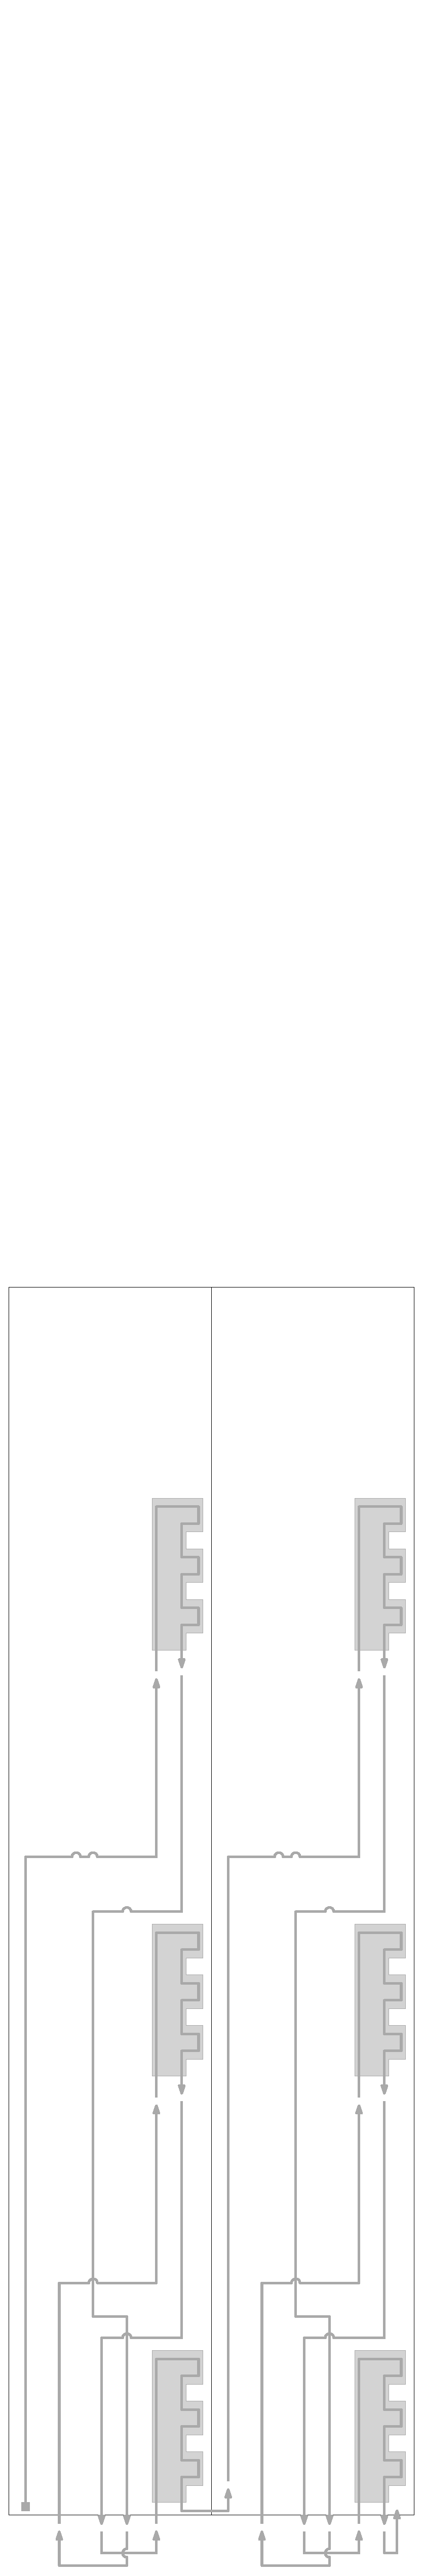
\includegraphics[width=0.6in]{counter_read_start_seed_case3_middle_level}
%         \caption{\label{fig:counter_read_start_seed_case3_middle_level} A ``clean'' counter row, before any reading has started.}
%     \end{subfigure}%
%     ~
%     \begin{subfigure}[t]{0.2\textwidth}
%         \centering
%         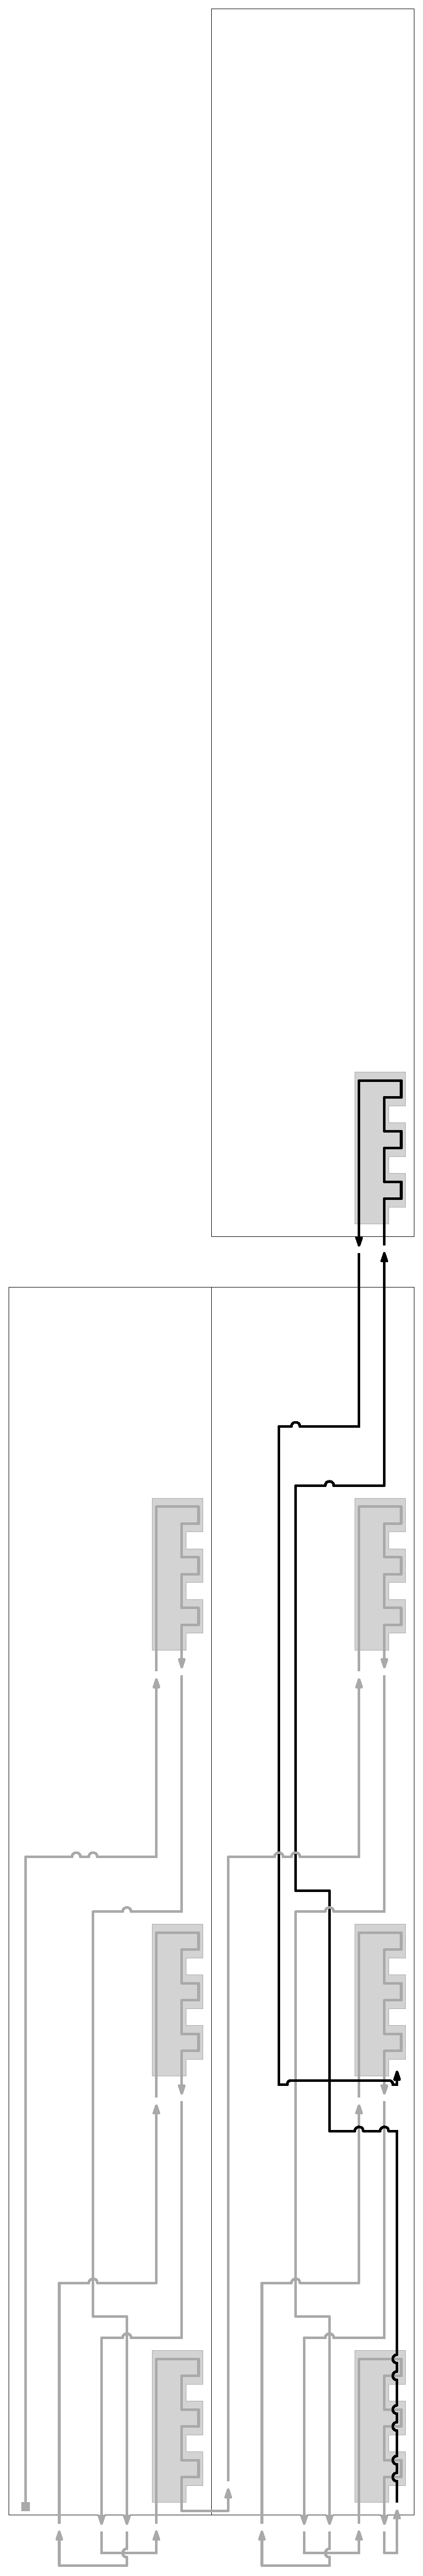
\includegraphics[width=0.6in]{counter_read_digit1_return_read_digit2_seed_case3_middle_level}
%         \caption{\label{fig:counter_read_digit1_return_read_digit2_seed_case3_middle_level} Reading digit 1, writing digit 1 in the next row, and returning to read digit 2 of the current row. }
%     \end{subfigure}%
%     ~
%     \begin{subfigure}[t]{0.2\textwidth}
%         \centering
%         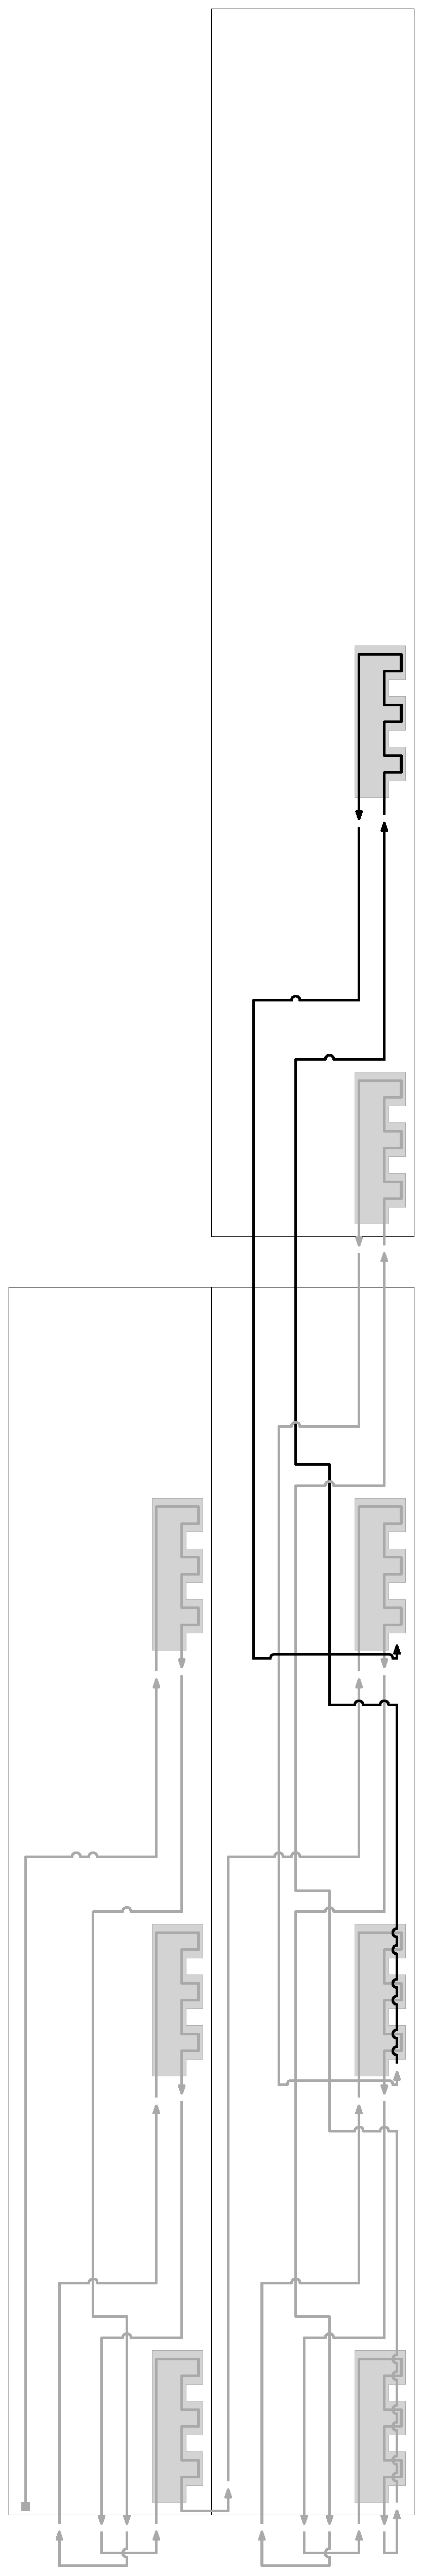
\includegraphics[width=0.6in]{counter_read_digit2_return_read_digit3_seed_case3_middle_level}
%         \caption{\label{fig:counter_read_digit2_return_read_digit3_seed_case3_middle_level} Reading digit 2, writing digit 2 in the next row, and returning to read digit 3 of the current row. }
%     \end{subfigure}%
%     ~
%     \begin{subfigure}[t]{0.2\textwidth}
%         \centering
%         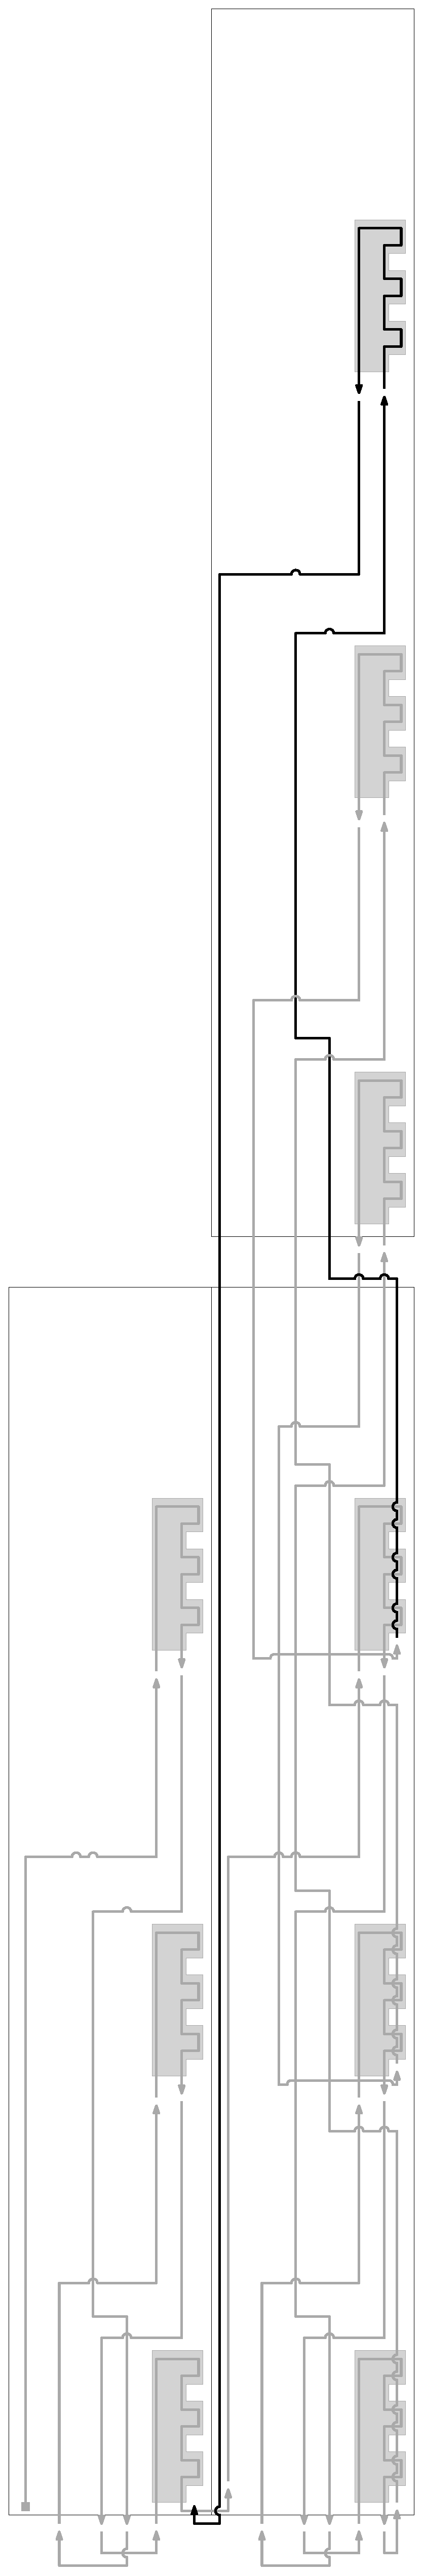
\includegraphics[width=0.6in]{counter_read_digit3_return_read_digit1_seed_case3_middle_level}
%         \caption{\label{fig:counter_read_digit3_return_read_digit1_seed_case3_middle_level} Reading digit 3, writing digit 3 in the next row, and returning to read digit 4 of the current row.}
%     \end{subfigure}%

%     \caption{\label{fig:counter_read_digit_return_read_digit_seed_case3} Progression of the counter as it reads the 3 least significant digits in one value, and writes the corresponding digits in the next row/value.}
% \end{figure}


\section{General counter}


\begin{figure}[H]
    \centering
    \begin{subfigure}[t]{0.2\textwidth}
        \centering
        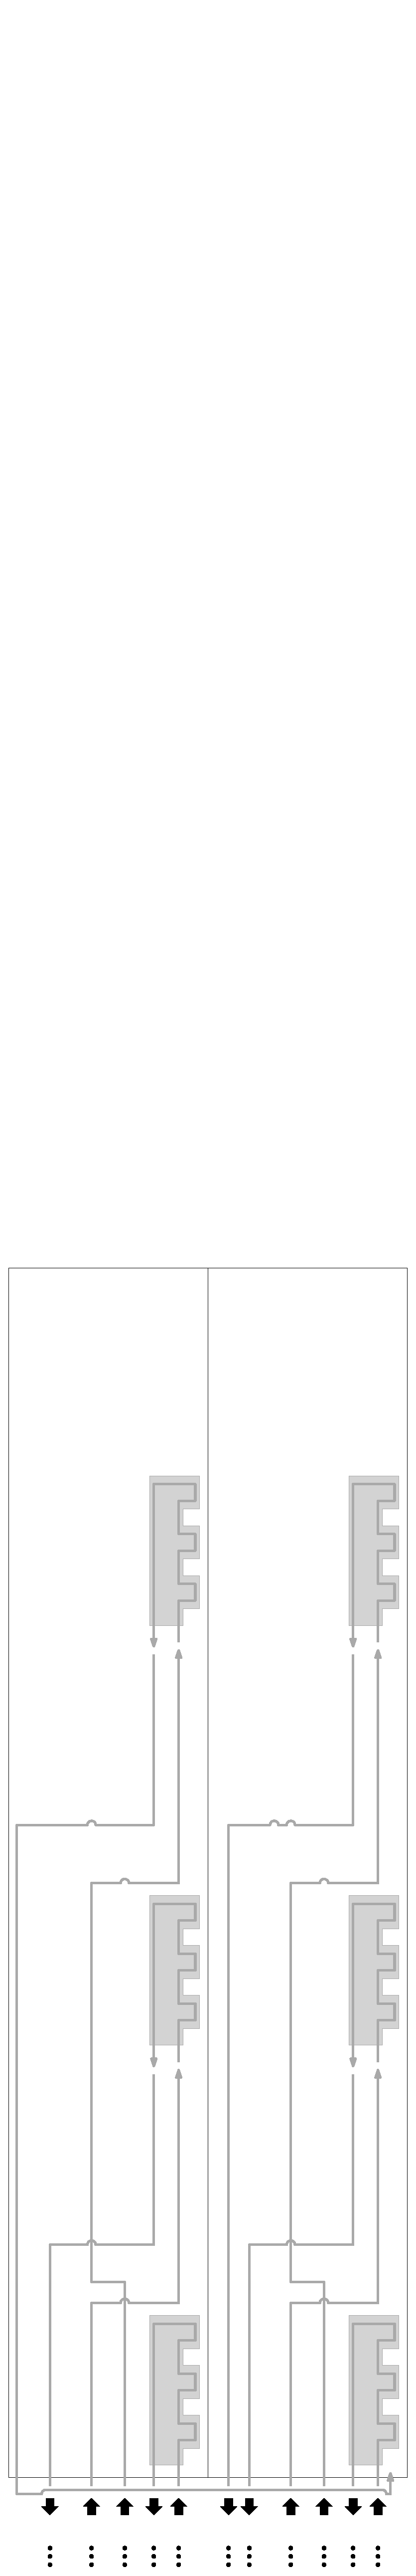
\includegraphics[width=0.6in]{counter_read_start_general_case3_middle_level}
        \caption{\label{fig:counter_read_start_general_case3_middle_level} A ``clean'' counter row, before any reading has started.}
    \end{subfigure}%
    ~
    \begin{subfigure}[t]{0.2\textwidth}
        \centering
        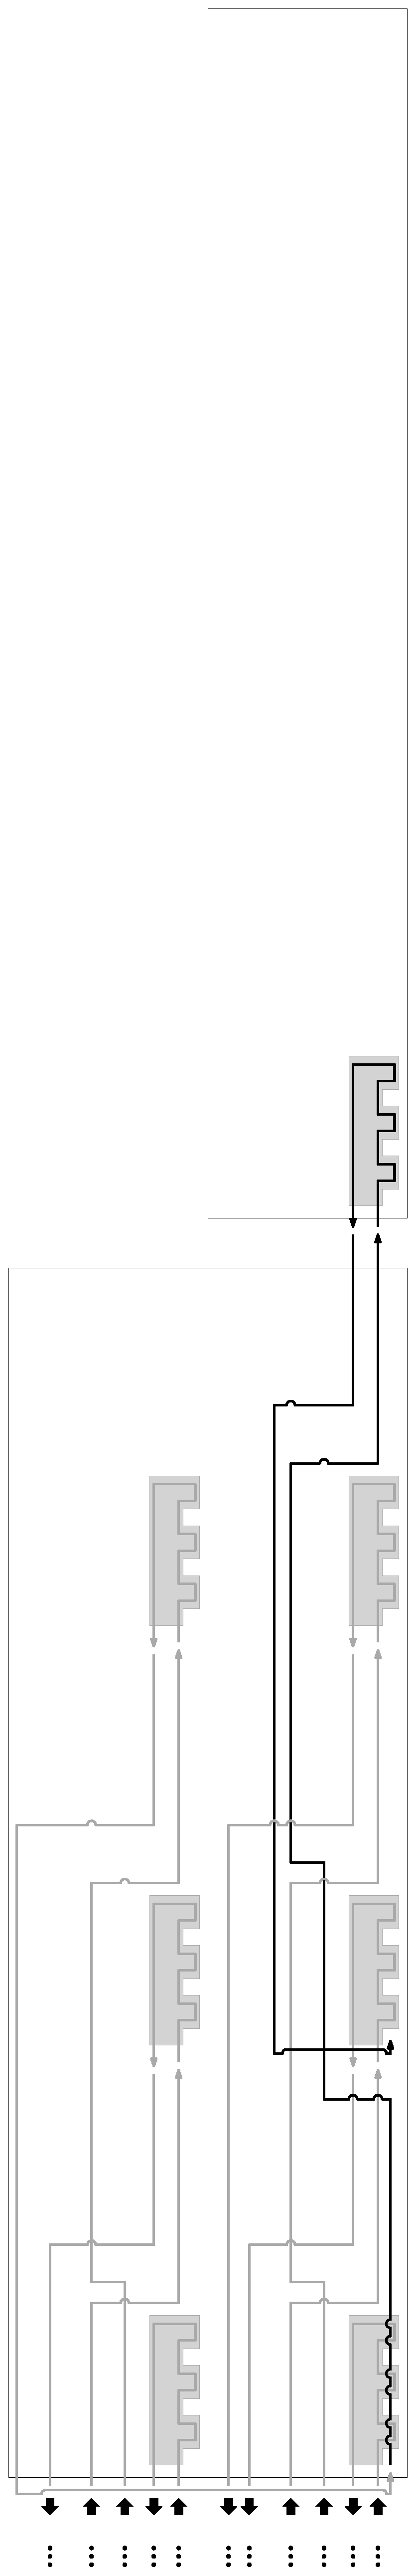
\includegraphics[width=0.6in]{counter_read_digit1_return_read_digit2_general_case3_middle_level}
        \caption{\label{fig:counter_read_digit1_return_read_digit2_general_case3_middle_level} Digit 1 in row $i$ is read, and row $i + 1$ is started. After this digit is
        written, the counter returns to row $i$, and is read to read digit 2.}
    \end{subfigure}%
    ~
    \begin{subfigure}[t]{0.2\textwidth}
        \centering
        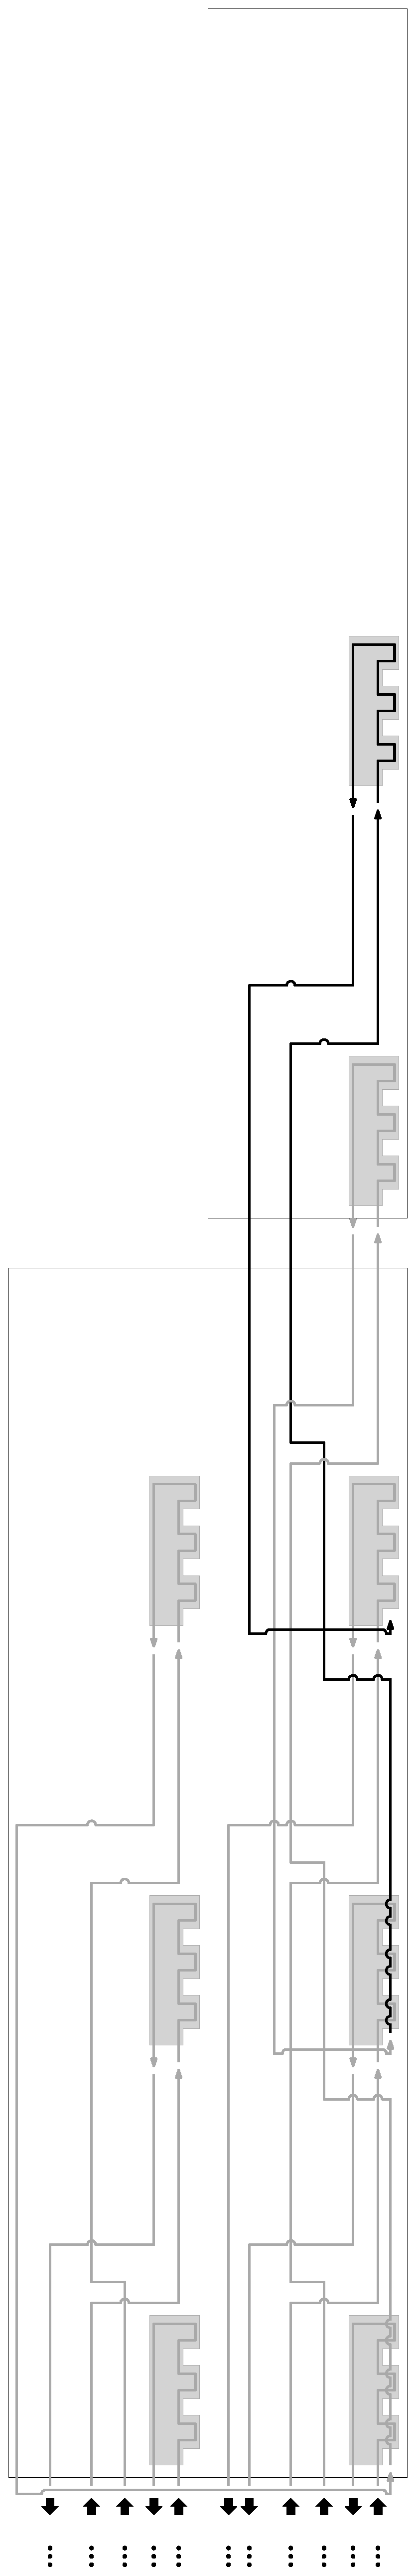
\includegraphics[width=0.6in]{counter_read_digit2_return_read_digit3_general_case3_middle_level}
        \caption{\label{fig:counter_read_digit2_return_read_digit3_general_case3_middle_level} Reading digit 2, writing digit 2 in the next row, and returning to read digit 3 of the current row. }
    \end{subfigure}%
    ~
    \begin{subfigure}[t]{0.2\textwidth}
        \centering
        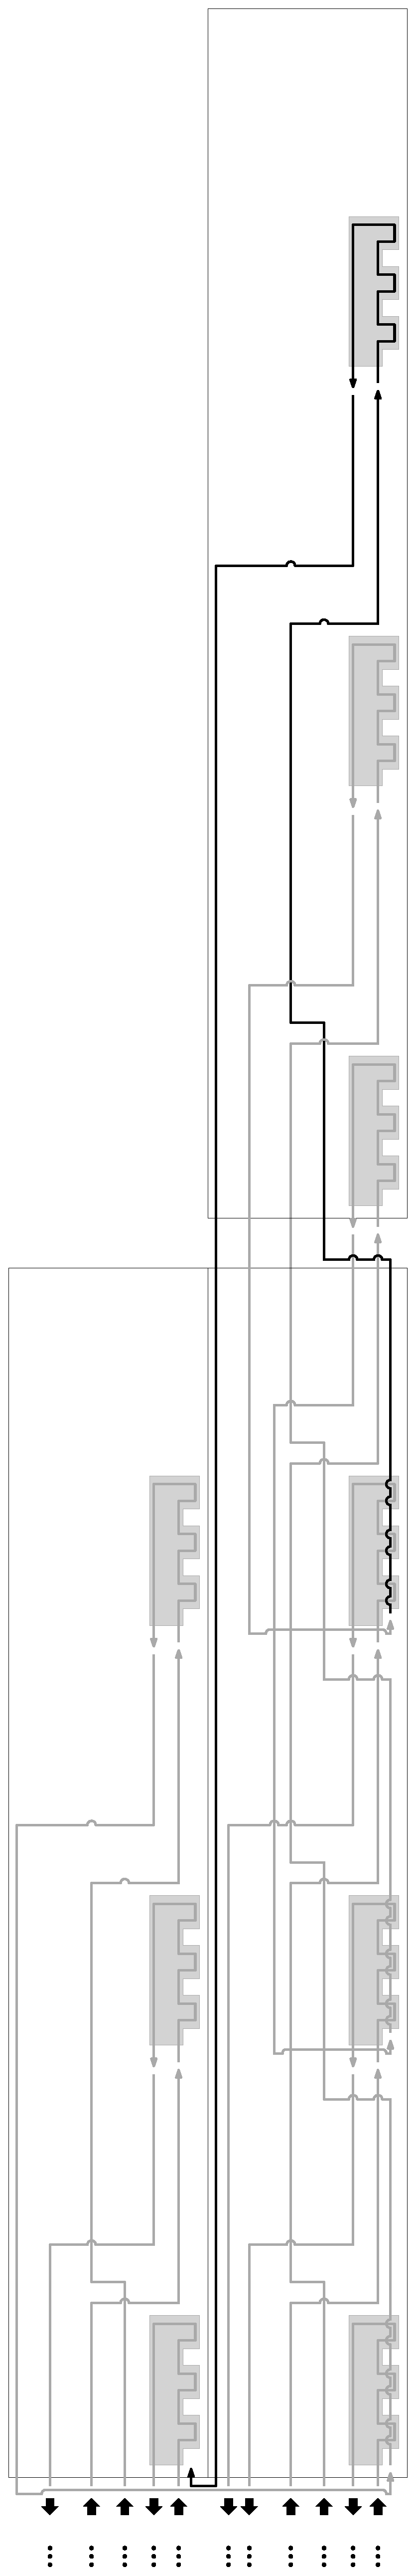
\includegraphics[width=0.6in]{counter_read_digit3_return_read_digit1_general_case3_middle_level}
        \caption{\label{fig:counter_read_digit3_return_read_digit1_general_case3_middle_level} Reading digit 3, writing digit 3 in the next row, and returning to read digit 4 of the current row.}
    \end{subfigure}%

    \caption{\label{fig:counter_read_digit_return_read_digit_general_case3}
    These illustrate how the counter reads and writes a digit region, in a general sense.
    The counter starts in the rightmost digit region, and reads the bottomost digit within
    that region. After reading digit 1, the corresponding digit region will be started in
    row $i + 1$. The counter writes the first digit, and then returns to digit 2 in row $i$.
    Once all the digits in the current digit region are read and written into row $i + 1$,
    the counter can then move to the next digit region in row $i$, begin reading row $i + 1$
    , or halt, depending on what signals are encoded in the geometry of the current row.}

\end{figure}

